\begin{pastexam}[label={px:ncku-111-prog-07}]{成大資訊聯招 111 學年度 第 7 題}
（複選）

\textbf{[2\%]} Consider the graph as follows. The DFS traversal is performed, starting from node 1. What are the potential sequences for the traversal?

\begin{center}
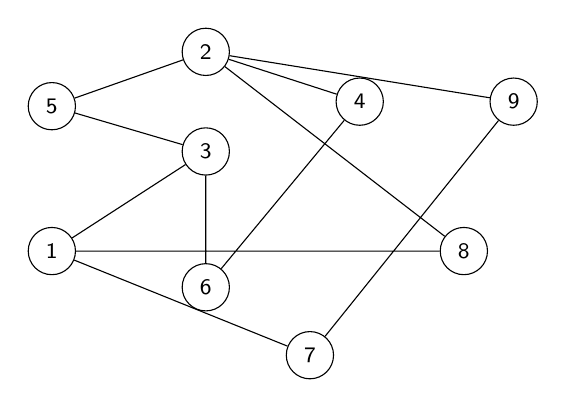
\begin{tikzpicture}[x=1.15cm,y=1.15cm,v/.style={circle,draw,inner sep=0pt,minimum size=6mm,font=\footnotesize\sffamily},s/.style={v,fill=black!25}]
\node[v] (n2) at (2.25,-0.7) {2};
\node[v] (n5) at (0.55,-1.3) {5};
\node[v] (n4) at (3.95,-1.25) {4};
\node[v] (n9) at (5.65,-1.25) {9};
\node[v] (n3) at (2.25,-1.8) {3};
\node[v] (n1) at (0.55,-2.9) {1};
\node[v] (n8) at (5.1,-2.9) {8};
\node[v] (n6) at (2.25,-3.3) {6};
\node[v] (n7) at (3.4,-4.05) {7};
\draw (n5)--(n2) (n5)--(n3) (n2)--(n4) (n2)--(n9) (n2)--(n8) (n3)--(n1) (n3)--(n6) (n4)--(n6) (n1)--(n8) (n1)--(n7) (n9)--(n7);
\end{tikzpicture}
\end{center}

(A) 1 7 9 2 4 6 3 5 8\\
(B) 1 3 6 4 2 5 9 7 8\\
(C) 1 7 8 3 5 6 4 2 9\\
(D) 1 8 2 4 6 3 5 9 7\\
(E) 1 2 5 6 4 2 9 7 8
\end{pastexam}

\begin{pastsoln}
答案：(A)、(B)、(D)。

\textbf{讀圖}。 從 $1$ 往右下的那條線擦過 $6$ 的下緣，終點是 $7$，是邊 $1$--$7$（$1$ 和 $6$、$6$ 和 $7$
都不相鄰）。 圖的鄰接關係：
\begin{center}
\begin{tabular}{c*{9}{c}}
\toprule
頂點 & 1 & 2 & 3 & 4 & 5 & 6 & 7 & 8 & 9 \\
\midrule
鄰居 & 3, 7, 8 & 4, 5, 8, 9 & 1, 5, 6 & 2, 6 & 2, 3 & 3, 4 & 1, 9 & 1, 2 & 2, 7 \\
\bottomrule
\end{tabular}
\end{center}

\textbf{判斷方法}（資結書第~21.4~節）。 DFS 的每一步：目前在 $u$，若 $u$ 還有沒拜訪的鄰居，下一個拜訪的
\textbf{必須}是其中之一；$u$ 的鄰居都拜訪過了，才退回 $u$ 的父節點繼續。 題目沒規定鄰居的順序，所以只要
每一步都符合這個規則，序列就「可能」出現。 檢查時維護一個堆疊（目前的路徑）。

\textbf{(A) 1 7 9 2 4 6 3 5 8}：$1 \to 7 \to 9 \to 2 \to 4 \to 6 \to 3 \to 5$，每一步都走到目前節點沒拜訪
的鄰居（$3$ 的鄰居 $1$、$6$ 已拜訪，只剩 $5$）。 $5$ 的鄰居 $2$、$3$ 都拜訪過，退回 $3$、$6$、$4$、$2$；$2$
還有 $8$ 沒拜訪，走到 $8$。 合法。

\textbf{(B) 1 3 6 4 2 5 9 7 8}：$1 \to 3 \to 6 \to 4 \to 2 \to 5$；$5$ 沒有未拜訪的鄰居，退回 $2$，走 $9$；
$9 \to 7$；$7$ 的鄰居 $1$、$9$ 都拜訪過，退回 $9$、$2$，$2$ 還有 $8$，走 $8$。 合法。

\textbf{(C) 1 7 8 3 5 6 4 2 9}：從 $7$ 出發時 $7$ 還有沒拜訪的鄰居 $9$，下一個必須是 $9$；何況 $7$ 和 $8$
根本不相鄰，而退回 $1$ 的前提是 $7$ 的鄰居都拜訪過。 不合法。

\textbf{(D) 1 8 2 4 6 3 5 9 7}：$1 \to 8 \to 2 \to 4 \to 6 \to 3 \to 5$；$5$ 沒有未拜訪的鄰居，退回 $3$
（鄰居 $1$、$5$、$6$ 都拜訪過）、$6$、$4$、$2$；$2$ 還有 $9$，走 $9$，再走 $9$ 的鄰居 $7$。 合法。

\textbf{(E) 1 2 5 6 4 2 9 7 8}：$2$ 出現兩次、$3$ 沒有出現，不是 $9$ 個頂點各拜訪一次；而且第一步
$1 \to 2$ 不是邊。 不合法。
\end{pastsoln}
